%%%%%%%%%%%%%%%%%%%%%%%%%%%%%%%%%%%
%This is the LaTeX ARTICLE template for RSC journals
%Copyright The Royal Society of Chemistry 2016
%%%%%%%%%%%%%%%%%%%%%%%%%%%%%%%%%%%

\documentclass[twoside,twocolumn,9pt]{article}
\usepackage{extsizes}
\usepackage[super,sort&compress,comma]{natbib} 
\usepackage[version=3]{mhchem}
\usepackage[left=1.5cm, right=1.5cm, top=1.785cm, bottom=2.0cm]{geometry}
\usepackage{balance}
\usepackage{times,mathptmx}
\usepackage{amsmath}
\usepackage{sectsty}
\usepackage{graphicx} 
\usepackage{lastpage}
\usepackage[format=plain,justification=justified,singlelinecheck=false,font={stretch=1.125,small,sf},labelfont=bf,labelsep=space]{caption}
\usepackage{float}
\usepackage{fancyhdr}
\usepackage{fnpos}
\usepackage[english]{babel}
\usepackage{array}
\usepackage{droidsans}
\usepackage{charter}
\usepackage[T1]{fontenc}
\usepackage[usenames,dvipsnames]{xcolor}
\usepackage{setspace}
\usepackage[compact]{titlesec}
\usepackage{hyperref}
%%%Please don't disable any packages in the preamble, as this may cause the template to display incorrectly.%%%


\usepackage{braket}

\usepackage{epstopdf}%This line makes .eps figures into .pdf - please comment out if not required.

\newcommand{\x}{\mathbf{r}}

\definecolor{cream}{RGB}{222,217,201}

\begin{document}

\pagestyle{fancy}
\thispagestyle{plain}
\fancypagestyle{plain}{

%%%HEADER%%%
\fancyhead[C]{\includegraphics[width=18.5cm]{head_foot/header_bar}}
\fancyhead[L]{\hspace{0cm}\vspace{1.5cm}\includegraphics[height=30pt]{head_foot/journal_name}}
\fancyhead[R]{\hspace{0cm}\vspace{1.7cm}\includegraphics[height=55pt]{head_foot/RSC_LOGO_CMYK}}
\renewcommand{\headrulewidth}{0pt}
}
%%%END OF HEADER%%%

%%%PAGE SETUP - Please do not change any commands within this section%%%
\makeFNbottom
\makeatletter
\renewcommand\LARGE{\@setfontsize\LARGE{15pt}{17}}
\renewcommand\Large{\@setfontsize\Large{12pt}{14}}
\renewcommand\large{\@setfontsize\large{10pt}{12}}
\renewcommand\footnotesize{\@setfontsize\footnotesize{7pt}{10}}
\makeatother

\renewcommand{\thefootnote}{\fnsymbol{footnote}}
\renewcommand\footnoterule{\vspace*{1pt}% 
\color{cream}\hrule width 3.5in height 0.4pt \color{black}\vspace*{5pt}} 
\setcounter{secnumdepth}{5}

\makeatletter 
\renewcommand\@biblabel[1]{#1}            
\renewcommand\@makefntext[1]% 
{\noindent\makebox[0pt][r]{\@thefnmark\,}#1}
\makeatother 
\renewcommand{\figurename}{\small{Fig.}~}
\sectionfont{\sffamily\Large}
\subsectionfont{\normalsize}
\subsubsectionfont{\bf}
\setstretch{1.125} %In particular, please do not alter this line.
\setlength{\skip\footins}{0.8cm}
\setlength{\footnotesep}{0.25cm}
\setlength{\jot}{10pt}
\titlespacing*{\section}{0pt}{4pt}{4pt}
\titlespacing*{\subsection}{0pt}{15pt}{1pt}
%%%END OF PAGE SETUP%%%

%%%FOOTER%%%
\fancyfoot{}
\fancyfoot[LO,RE]{\vspace{-7.1pt}\includegraphics[height=9pt]{head_foot/LF}}
\fancyfoot[CO]{\vspace{-7.1pt}\hspace{13.2cm}\includegraphics{head_foot/RF}}
\fancyfoot[CE]{\vspace{-7.2pt}\hspace{-14.2cm}\includegraphics{head_foot/RF}}
\fancyfoot[RO]{\footnotesize{\sffamily{1--\pageref{LastPage} ~\textbar  \hspace{2pt}\thepage}}}
\fancyfoot[LE]{\footnotesize{\sffamily{\thepage~\textbar\hspace{3.45cm} 1--\pageref{LastPage}}}}
\fancyhead{}
\renewcommand{\headrulewidth}{0pt} 
\renewcommand{\footrulewidth}{0pt}
\setlength{\arrayrulewidth}{1pt}
\setlength{\columnsep}{6.5mm}
\setlength\bibsep{1pt}
%%%END OF FOOTER%%%

%%%FIGURE SETUP - please do not change any commands within this section%%%
\makeatletter 
\newlength{\figrulesep} 
\setlength{\figrulesep}{0.5\textfloatsep} 

\newcommand{\topfigrule}{\vspace*{-1pt}% 
\noindent{\color{cream}\rule[-\figrulesep]{\columnwidth}{1.5pt}} }

\newcommand{\botfigrule}{\vspace*{-2pt}% 
\noindent{\color{cream}\rule[\figrulesep]{\columnwidth}{1.5pt}} }

\newcommand{\dblfigrule}{\vspace*{-1pt}% 
\noindent{\color{cream}\rule[-\figrulesep]{\textwidth}{1.5pt}} }

\makeatother
%%%END OF FIGURE SETUP%%%

\newcommand{\filipp}[1]{{\color{red} #1}}
\newcommand{\guo}[1]{{\color{blue} #1}}
\newcommand{\brian}[1]{{\color{purple} #1}}

%%%TITLE, AUTHORS AND ABSTRACT%%%
\twocolumn[
  \begin{@twocolumnfalse}
\vspace{3cm}
\sffamily
\begin{tabular}{m{4.5cm} p{13.5cm} }

\includegraphics{head_foot/DOI} & \noindent\LARGE{\textbf{Size
    dependence of noncovalent interactions within the random phase
    approximation$^\dag$}} \\%Article title goes here instead of the
                             %text "This is the title" 
\vspace{0.3cm} & \vspace{0.3cm} \\

 & \noindent\large{
Brian D. Nguyen\textit{$^{a}$}, Matthew M. Agee\textit{$^{a}$}, Asbj{\"o}rn
   M. Burow\textit{$^{a}$}\textit{$^{\ddag}$}, Guo
   P. Chen\textit{$^{a}$}, Filipp Furche,$^{\ast}$\textit{$^{a}$}}
 \\%Author names go here instead of "Full name", etc. 

\includegraphics{head_foot/dates} & \noindent\normalsize{
Accurate predictions of noncovalent interaction (NI) effects in
large and complex chemical systems remain challenging for 
electronic structure theory. Here we assess the performance of the
random phase approximation (RPA) to the ground state correlation energy
in capturing NIs for large supramolecular complexes contained in the
S30L benchmark [Sure, \textit{J. Chem. Theory Comput.}, 2015, \textbf{11(8)},
3785-3801]. The RPA interaction energies agree with the benchmark data within
$\sim$10$\%$, close to the intrinsic accuracy of the benchmark. The quality of
RPA interaction energies is found to be independent of the system size, unlike
that of second-order M{\o}ller-Plesset perturbation theory or semilocal
density functional approximations (DFAs). This supports the notion that
beyond-pairwise NIs are critically important even in moderately large
molecules with 100-200 atoms. Comparison of rotational constants obtained
from RPA structure optimizations to gas phase spectroscopic data
[Risthaus \textit{et al.}, \textit{J. Chem. Theory Comput.}, 2013, \textbf{9}, 1580]
indicates that the performance of RPA for intramolecular NIs is also
system-size independent. The accuracy of the RPA rotational
constants is comparable to the one obtained with of the most
sophisticated empirical DFAs.
 } \\%The abstrast goes here instead of the text
                         %"The abstract should be..." 

\end{tabular}

 \end{@twocolumnfalse} \vspace{0.6cm}

  ]
%%%END OF TITLE, AUTHORS AND ABSTRACT%%%

%%%FONT SETUP - please do not change any commands within this section
\renewcommand*\rmdefault{bch}\normalfont\upshape
\rmfamily
\section*{}
\vspace{-1cm}


%%%FOOTNOTES%%%

\footnotetext{\textit{$^{a}$~University of California, Irvine,
    Department of Chemistry, 1102 Natural Sciences II, Irvine, CA
    92697-2025, USA; E-mail: filipp.furche@uci.edu}}
%\footnotetext{\textit{$^{b}$~Address, Address, Town, Country. }}

%Please use \dag to cite the ESI in the main text of the article.
%If you article does not have ESI please remove the the \dag symbol from the title and the footnotetext below.
\footnotetext{\dag~Electronic Supplementary Information (ESI) available: [details of any supplementary information available should be included here]. See DOI: 10.1039/b000000x/}
%additional addresses can be cited as above using the lower-case letters, c, d, e... If all authors are from the same address, no letter is required

\footnotetext{\ddag~Present address: Ludwig-Maximilians-Universit\"at M\"unchen, Department of Chemistry, Butenandtstr. 7, D-81377 M\"unchen, Germany}


%%%END OF FOOTNOTES%%%

%%%MAIN TEXT%%%%
% The main text of the article\cite{Mena2000} should appear here.

% \subsection{This is the subsection heading style}
% Section headings can be typeset with and without numbers.\cite{Abernethy2003}

% \subsubsection{This is the subsubsection style.~~} These headings should end in a full point.  

% \paragraph{This is the next level heading.~~} For this level please use \texttt{\textbackslash paragraph}. These headings should also end in a full point.

% \section{Graphics and tables}
% \subsection{Graphics}
% Graphics should be inserted on the page where they are first mentioned (unless they are equations, which appear in the flow of the text).\cite{Cotton1999}

% \begin{figure}[h]
% \centering
%   \includegraphics[height=3cm]{example1}
%   \caption{An example figure caption \textendash\ the image is from the \textit{Physical Chemistry Chemical Physics} cover gallery.}
%   \label{fgr:example}
% \end{figure}

% \begin{figure*}
%  \centering
%  \includegraphics[height=3cm]{example2}
%  \caption{An image from the \textit{Physical Chemistry Chemical Physics} cover gallery, set as a two-column figure.}
%  \label{fgr:example2col}
% \end{figure*}

% \subsection{Tables}
% Tables typeset in RSC house style do not include vertical lines. Table footnote symbols are lower-case italic letters and are typeset at the bottom of the table. Table captions do not end in a full point.\cite{Arduengo1992,Eisenstein2005}

%\begin{table}[h]
%\small
%  \caption{\ An example of a caption to accompany a table}
%  \label{tbl:example}
%  \begin{tabular*}{0.48\textwidth}{@{\extracolsep{\fill}}lll}
%    \hline
%    Header one (units) & Header two & Header three \\
%    \hline
%    1 & 2 & 3 \\
%    4 & 5 & 6 \\
%    7 & 8 & 9 \\
%    10 & 11 & 12 \\
%    \hline
%  \end{tabular*}
%\end{table}

% Adding notes to tables can be complicated.  Perhaps the easiest method is to generate these manually.\footnote[4]{Footnotes should appear here. These might include comments relevant to but not central to the matter under discussion, limited experimental and spectral data, and crystallographic data.}

% \begin{table*}
% \small
%   \caption{\ An example of a caption to accompany a table \textendash\ table captions do not end in a full point}
%   \label{tbl:example}
%   \begin{tabular*}{\textwidth}{@{\extracolsep{\fill}}lllllll}
%     \hline
%     Header one & Header two & Header three & Header four & Header five & Header six  & Header seven\\
%     \hline
%     1 & 2 & 3 & 4 & 5 & 6  & 7\\
%     8 & 9 & 10 & 11 & 12 & 13 & 14 \\
%     15 & 16 & 17 & 18 & 19 & 20 & 21\\
%     \hline
%   \end{tabular*}
% \end{table*}

% \section{Equations}

% Equations can be typeset inline \textit{e.g.}\ $ y = mx + c$ or displayed with and without numbers:

%  \[ A = \pi r^2 \]

% \begin{equation}
%   \frac{\gamma}{\epsilon x} r^2 = 2r
% \end{equation}

% You can also put lists into the text. You can have bulleted or numbered lists of almost any kind. 
% The \texttt{mhchem} package can also be used so that formulae are easy to input: \texttt{\textbackslash ce\{H2SO4\}} gives \ce{H2SO4}. 

% For footnotes in the main text of the article please number the footnotes to avoid duplicate symbols. \textit{e.g.}\ \texttt{\textbackslash footnote[num]\{your text\}}. The corresponding author $\ast$ counts as footnote 1, ESI as footnote 2, \textit{e.g.}\ if there is no ESI, please start at [num]=[2], if ESI is cited in the title please start at [num]=[3] \textit{etc.} Please also cite the ESI within the main body of the text using \dag.

% \section{Conclusions}
% The conclusions section should come at the end of article. For the reference section, the style file \texttt{rsc.bst} can be used to generate the correct reference style.

% \section*{Conflict of interest}
% Please confirm you have read our policy on \href{http://www.rsc.org/journals-books-databases/journal-authors-reviewers/author-responsibilities/#code-of-conduct}{Conflict of interest} and that a conflict of interest statement is included in your manuscript.  Please note that this statement is required for all submitted manuscripts.  If no conflicts exist, please state that ``There are no conflicts to declare'' under this ``Conflict of interest'' heading after the conclusions section.
% %%%END OF MAIN TEXT%%%

\section{Introduction}

While covalent bonding is a central paradigm of chemical theory,
noncovalent interactions
(NIs)\cite{HobzaCollectCzechChemCommun, Dobson12JPhysCondensMatter24p073201}
have long been 
considered less important. In small molecules, NIs are at least one
order of magnitude weaker than covalent bonds, and their low chemical
specificity make them difficult to detect and control. However, NIs
grow nonadditively with system size due to their long
range.\cite{DobsonIntJQuantumChem} 
Indeed, NIs often determine conformation, tertiary 
structure, and other properties of molecular
aggregates and complexes,\cite{Huang16Langmuir32p12352,
  Biedermann16ChemRev116p5216, Britz06ChemSocRev35p637}
materials,\cite{Liu13AdvMater25p1521, Georgakilas16ChemRev116p5464}
or molecular crystals.\cite{Moulton01ChemRev101p1629, 
  Beran16ChemRev116p5567}
Recent advances in experimental techniques such as molecular beam
spectroscopy\cite{Becucci16ChemRev116p5014}
have made NIs observable, and even areas focused on 
covalent bonding such as synthetic chemistry and catalysis
increasingly use NIs to fine-tune reactivity and selectivity.
\cite{Zuend09JAmChemSoc131p15358, Tao16ChemEurJ22p8786}

Electronic structure methods have been traditionally developed and
tested for small molecules. A key assumption underlying this ``bottom-up''
approach is that methods performing well for small systems may be scaled
up to larger ones without deterioration in accuracy. While size
consistency \cite{Bartlett77IntJQuantumChem12p165}
is usually sufficient to
ensure that the accuracy of covalent interactions is independent
of the system size, recent work by Grimme and co-workers showed that
this assumption is not justified for NIs: While second-order
M{\o}ller-Plesset perturbation theory (MP2) and semilocal density
functional approximations (DFAs) with empirical two-body dispersion
corrections\cite{Grimme06JComputChem27p1787} accurately describe NIs
in small molecules, their performance severely deteriorates for systems
containing over $100$ atoms\cite{Grimme12ChemEurJ18p9955}. This has been
ascribed to missing three- and higher-body dispersion interactions in
these methods, and the success of subsequently developed corrections
including three- and higher-body dispersion effects such as 
D3,\cite{Grimme12ChemEurJ18p9955} D4,\cite{Caldeweyher17JChemPhys147p034112}
% \guo{(Shall we also cite the D4 paper 10.1063/1.4993215 ?)} \filipp{yes}
and the many-body dispersion
methods \cite{Tkatchenko12PhysRevLett108p236402} seems to support this
conclusion.

The random phase approximation (RPA) to the ground-state correlation
energy\cite{Langreth75SolidStateCommun17p1425,
Langreth77PhysRevB15p2884} arises from interactions between
virtual ground-state density fluctuations,\cite{Bohm53PhysRev92p609,
Furche08JChemPhys129p114105}
making RPA a method of
choice for describing NIs from a theoretical perspective.
\cite{Dobson05IntJQuantumChem101p579, Dobson12JPhysCondensMatter24p073201}
RPA is nonempirical and
dispersion consistent, yielding seamless potential energy surfaces.
The RPA correlation energy captures three- and higher-body dispersion
effects because it correctly includes polarization and
screening.\cite{Chen17AnnuRevPhysChem68p421}
The accuracy of RPA is
largely independent of the gap between highest molecular orbital (HOMO)
and the lowest unoccupied molecular orbital (LUMO) energies, permitting
applications to open-shell compounds and transition-metal or $f$-element
complexes. \filipp{10.1021/om500624x +  10.1021/acs.jctc.6b00756}

The accuracy of RPA for NIs in small molecules
\cite{Eshuis11JPhysChemLett2p983}, rare-gas solids
\cite{Harl09PhysRevLett103p056401} and layered materials \filipp{https://doi.org/10.1103/PhysRevLett.105.196401} is well 
documented, but whether it is transferable to intra- and supramolecular NIs is
unclear. Enabled by efficient RPA energy
\cite{Eshuis10JChemPhys132p234114} and analytic derivatives
\cite{Burow14JChemTheoryComput10p180} 
implementations, we investigate this question by assessing RPA energies and 
structures using Grimme's S30L and Rot34 benchmarks. S30L contains
noncovalently bound supramolecular complexes with 86-177 atoms and
binding energies between -29.0 and -131.5 kcal/mol. Rot34, on the other
hand, contains 34 rotational constants from gas phase experiments
serving as a sensitive probe for structures and intramolecular
NIs. 

% Within RPA, electron correlation arises from interactions between
% virtual ground-state density fluctuations. RPA is dispersion consistent,
% produces seamless potential energy surfaces,
% and because it correctly includes polarization and
% screening,\cite{Chen17AnnuRevPhysChem68p421} three- and
% higher-body dispersion effects are captured. The accuracy of RPA is
% largely independent of the gap between highest molecular orbital (HOMO)
% and the lowest unoccupied molecular orbital (LUMO) energies, permitting
% applications to open-shell compounds and transition- or $f$-element
% complexes where MP2 fails. Recent alogrithmic improvements have made RPA
% calculations affordable for systems with hundreds of
% atoms\cite{Eshuis10JChemPhys132p234114,Kaltak14PhysRevB90p054115,
%   Bleiziffer13JChemPhys139p084113};
% the cost of an RPA calculation is only a few times that
% of a SOS-MP2 calculation.\cite{Grimme16PhysChemChemPhys}

% The increasing need to accurately model noncovalent interaction has
% been a driver for the development of new theoretical and computational
% methods. It is now widely accepted that the popular semi-local density
% functional approximations (DFAs) fundamentally lack the ability to
% capture long-range dispersion\cite{Grimme06JChemPhys124p034108,
%   Kristyan94ChemPhysLett229p175}. Empirical dispersion corrections pioneered by
% Grimme and co-workers\cite{Grimme12ChemEurJ18p9955} combined with
% semilocal DFAs can be suprisingly accurate and come at virtually no
% additional cost, but require adjustment for each atom and functional,
% and occasionally fail\cite{Ilawe15JChemTheoryComput11p5426}, particularly
% for polarizable systems\cite{Kim16JPhysChemLett}. Other corrections such as
% Thakchenko-Scheffler\cite{Tkatchenko09PhysRevLett102p073005},
% many-body dispersion\cite{Tkatchenko12PhysRevLett108p236402} methods, the
% Becke-Johnson model\cite{Becke05JChemPhys122p154104,Becke07JChemPhys127p154108},
% Tao-Perdew $C_{6}$ coefficient\cite{Tao12ProcNatlAcadSciUSA}, van der Waals
% functionals \cite{Andersson96PhysRevLett76p102}
% include information from the electron density but face similar
% challenges. Correcting the quite erratic behavior of many DFAs for
% slightly overlapping densities and open-shell systems is especially
% difficult. \filipp{mention ECPs} \cite{Zhao08TheorChemAcc120p215}

% Second-order M{\o}ller-Plesset (MP2) perturbation theory, qualitatively
% includes long-range dispersion\cite{Riley12JPhysChemA116p4159}, but
% suffers from a lack of ``dispersion consistency''\cite{Toulouse13JChemPhys},
% yielding C6 coefficients at the uncoupled Hartree-Fock (HF) level.
% This has prompted the development of approaches such as
% MP2C\cite{Pitonak10JChemTheoryComput}, which explicitly replace the
% long-range part of the MP2 potential energy with more accurate potentials
% from coupled HF calculations, or even D3 corrections\cite{Grimme12ChemEurJ18p9955}.
% However, these approaches are not ``seamless'',
% i.e., they require ``stitching together'' the potential energy surface
% using different methods, introducing empiricism and limiting predictive
% power; the same limitation applies to symmetry adapted perturbation theory,
% arguably the most accurate method available for modeling noncovalent
% interactions. On the other hand the performance of MP2 also deteriorates
% significantly with system size, probably  due to lacking three- and
% higher-body dispersion\cite{Sherrill09RevCompChem26p1}. Coupled cluster
% singles doubles  with perturbative triples (CCSD(T)) yields highly
% accurate non-covalent interaction energies, but remains prohibitively
% expensive for many applications, despite recent algorthimic
% advances.\cite{Hattig10JChemPhys,Rolik13JChemPhys,Riplinger13JChemPhys}

\section{Theory}

\subsection{Statement of the Problem}

We consider a system consisting of two subsystems A and B separated by a
distance $R$ with scaled interaction $\alpha \hat{H}_{\text{AB}}$. The
supersystem Hamiltonian at coupling strength $\alpha$ is
\begin{equation}
  \hat{H}_{\alpha}(R) = \hat{H}_{\text{A}} + \hat{H}_{\text{B}} + \alpha
  \hat{H}_{\text{AB}}(R),
\end{equation}
where $\hat{H}_{\text{A}}$ and $\hat{H}_{\text{B}}$ denote the
Hamiltonians of the fragments A and B at full coupling. The physical
Hamiltonian of the supersystem thus corresponds to $\alpha = 1$.

The interaction energy of the fragments A and B is the difference
between the ground state energies at full and zero coupling,
\begin{equation}
  E_{\text{AB}}(R) = E_{\alpha 0}(R)|_{\alpha=1} - E_{\alpha 0}|_{\alpha=0},
\end{equation}
which may be reexpressed as a coupling strength integral via the
Hellmann-Feynman theorem,
\begin{equation}
  E_{\text{AB}}(R) = \int_0^1 d\alpha \frac{d}{d \alpha} E_{\alpha 0}(R)
  = \int_0^1 d \alpha \braket{\Psi_{\alpha
      0}|\hat{H}_{\text{AB}}(R)|\Psi_{\alpha 0}}.
\end{equation}
The wavefunctions $\ket{\Psi_{\alpha n}}$ and energies $E_{\alpha n}$
are solutions of the stationary Schr{\"o}dinger equation
\begin{equation}
  \hat{H}_{\alpha}(R) \ket{\Psi_{\alpha n}} =  E_{\alpha n}
  \ket{\Psi_{\alpha n}}.
\end{equation}
We shall assume that the ground state wavefunction $\Psi_{\alpha 0}$ is
square integrable and nondegenerate for $0 \leq \alpha \leq 1$. The
interaction energy may thus be expressed as
\begin{equation}
  E_{\text{AB}}(R) = E^{(1)}_{\text{AB}}(R) + E^{\text{C}}_{\text{AB}}(R),
\end{equation}
where $E^{(1)}_{\text{AB}}(R) = \braket{\Psi_{0 0}|\hat{H}_{\text{AB}}|
  \Psi_{0 0}}$ is the first-order interaction energy and all
higher orders in $\alpha$ are gathered in the remaining correlation
part of the interaction energy. For large intermolecular distances $R$,
the overlap between the two subsystem ground-state wavefunctions decays
as $e^{-\gamma R}$, where 
the exponent $\gamma$ is related to the subsystem ionization potentials
$I_A$ and $I_B$ via $\gamma = \sqrt{I_A} + \sqrt{I_B}$
\filipp{check}. As a result, exchange contributions to the interaction
energy resulting from antisymmetry of the total wavefunction under
permutation of electrons between $A$ and $B$ decay exponentially. Thus,
to $O(e^{-\gamma R})$, the first-order interaction energy is the
electrostatic interaction (Hartree) energy of the combined nuclear and
electronic charge densities of subsystems A and B, and
\begin{equation}
  E^{\text{C}}_{\text{AB}}(R) = \int_0^1
  d\alpha \int_{-\infty}^{\infty} \frac{d\omega}{2 \pi}  \int dx_A
  dx_B \frac{ 
    \chi_{\alpha}(\omega,x_A,x_B) - \chi_{0}(\omega,x_A,x_B) }{
    |\x_A-\x_B+\mathbf{R}|} + E^{\text{C pol}}_{\text{AB}}(R) + O(e^{-\gamma R}).
\end{equation}
$\chi_{\alpha}$ is the frequency-dependent intersystem density-density
response function, i.e.,
\begin{equation}
  \chi_{\alpha}(\omega,x_A,x_B) = - \sum_{n \ne 0} \left( \frac{
      \braket{\Psi_{\alpha 0}| \hat{\rho}(x_A) | \Psi_{\alpha n}}
      \braket{\Psi_{\alpha n}| \hat{\rho}(x_B) | \Psi_{\alpha 0}} }{
      \omega - (E_{\alpha n} - E_{\alpha 0}) } - \frac{
      \braket{\Psi_{\alpha 0}| \hat{\rho}(x_B) | \Psi_{\alpha n}}
      \braket{\Psi_{\alpha n}| \hat{\rho}(x_A) | \Psi_{\alpha 0}} }{
      \omega + (E_{\alpha n} - E_{\alpha 0}) } \right).
\end{equation}
$E^{\text{C pol}}_{\text{AB}}(R)$ accounts for changes in the
electrostatic energy due to polarization,
\begin{equation}
  E^{\text{C pol}}_{\text{AB}}(R) = \int_0^{1} d\alpha \int dx_A dx_B
  \frac{ \tilde{\rho}_{\alpha}(x_A) \tilde{\rho}_{\alpha}(x_B) }{|\x_A
    -\x_B -\mathbf{R}|},
\end{equation}
where $\tilde{\rho}_{\alpha}(x) = \rho_{\alpha}(x) - \rho_0(x)$ accounts
for the change in the total electron and nuclear density due to the
interaction. 


\section{Methods}
\subsection{Computational Details}

RPA energies and analytic derivatives were obtained in a post-Kohn-Sham (KS)
fashion, i.e., a KS calculation using a semilocal DFA was first performed
to obtain the KS orbitals, and subsequently the exact exchange energy
and the RPA correlation energy were evaluated non-selfconsistently. The
PBE\cite{Perdew96PhysRevLett77p3865} and TPSS\cite{Tao03PhysRevLett91p146401}
DFAs were used for the KS calculations along with ultrafine grids (size
m5\cite{Treutler95JChemPhys102p346}). The resolution-of-the-identity 
(RI) approximation and imaginary frequency integration were
employed for the RPA correlation energy evaluation as implemented in
the \textsc{Rirpa} module\cite{Eshuis10JChemPhys132p234114} of \textsc{Turbomole 7.0}.
\cite{Furche14WIREsComputMolSci4p91} The performance of RPA to predict
NIs and intramolecular interactions was benchmarked against the
S30L and ROT34 test sets.

Single-point RPA calculations were computed on complexes from the S30L set
using 100 frequency gridpoints and frozen core approximation. The complete
basis set (CBS) limit of the RPA correlation energy was estimated using two-point
$1/X^3$ extrapolation, where $X$ is the cardinal number\cite{Eshuis12JChemPhys136p084105,
Halkier98ChemicalPhysicsLetters286p243}. Dunning's correlation-consistent
polarized triple and quadruple $\zeta$ valence basis sets, cc-pVTZ and
cc-pVQZ \cite{Dunning89JChemPhys90p1007}, were employed for the extrapolation as
a balance between efficiency and accuracy. The energy expectation value of the KS
determinant was computed using Karlsruhe polarized quadruple $\zeta$ valence basis
sets (def2-QZVP\cite{Weigend05PhysChemChemPhys7p3297}), which are better suited for
density functional calculations than the Dunning's basis set\cite{Weigend03JChemPhys119p12753}.
Auxiliary basis sets optimized for the corresponding primary basis sets were
employed in the \textsc{Rirpa} calculations\cite{Weigend02JChemPhys116p3175}. %\filipp{Ref. cbasen} 
The basis set superposition error (BSSE) was treated with 50\% counterpoise
correction as recommended by Risthaus and coworkers.\cite{Risthaus13JChemTheoryComput9p1580,
Eshuis12JChemPhys136p084105}. Errors in RPA interaction energies are
computed as $E_{\text{RPA}}-E_{\text{Ref}}$, where $E_{\text{Ref}}$ is the reference
interaction energy.

%\filipp{Please also define rMinMax error here.}

For the ROT34 benchmark, RPA geometry optimizations were converged to a
maximum gradient norm of $10^{-4}$ a.u. or less. All electrons were
correlated and a fine frequency grid with 200 grid points was employed
for the RPA energy and gradient calculations. The Ahlrichs and coworker
def2-TZVP and def2-QZVP basis sets\cite{Weigend05PhysChemChemPhys7p3297}
were reported for comparison. Statistical data such as mean absolute error (MAE),
mean error (ME), signed relative standard deviation (SD), and relative
Min-Max (rMinMax) error in percentage was computed for both benchmarks.
The rMinMax error is the relative difference between the maximum and
minimum errors.

%from your plots? If so, please state it here and explain why.}
% \guo{Combine this paragraph with the next two.} 
% For comparison, results obtained using the def2-TZVP
%  and def2-QZVP
%  basis sets are presented as well.
% Tight convergence of the RPA geometry optimization used 200 imaginary
% frequency integration points\cite{Eshuis10JChemPhys132p234114},
% density convergence of 10$^{-7}$ a.u, self-consistent field convergence
% of 10$^{-7}$.
%The computed rotational constants are compared to the
%experimental results ($B_{\text{e}}$) and the error is defined to
%be $B_{\text{e}} - B_{\text{calc}}$.
% \guo{Brian, error should be defined as the calculated value minus the experimental
% value, not the other way around. Please double check the result section to make sure
% the errors were calculated correctly.}

 \subsection{Basis set convergence}
% The RPA interaction energy of the S30L test set\cite{Grimme12ChemEurJ18p9955,
%   Risthaus13JChemTheoryComput9p1580} used 100 imaginary frequency
% integration points\cite{Eshuis10JChemPhys132p234114}. Interaction energy
% was computed using converged PBE\cite{Perdew96PhysRevLett77p3865} and
% TPSS\cite{Tao03PhysRevLett91p146401} molecular orbitals together
% with the two-point extrapolation scheme based on the universal cusp
% condition\cite{Eshuis12JChemPhys136p084105},
% \begin{equation}
%   E_{XY}^{\infty} = \frac{E_X X^3 - E_y Y^3}{X^3 - Y^3} 
% \end{equation}
% where X and Y are the cardinal numbers of the basis set used to
% compute the RPA correlation energies $E_{X}$ and $E_{Y}$.
% The triple-$\zeta$ and quadruple-$\zeta$ extrapolation
% \cite{Eshuis12JChemPhys136p084105} was consistently applied to
% the RPA correlation energy with the Dunning basis set while the
% Hartree Fock Exchange (HXX) energy was computed with def2-QZVP basis
% \cite{Weigend03JChemPhys119p12753}. At the basis set limit, the
% suggested $50\%$ CP correction is reasonable to account for the
% basis set superposition error (BSSE)\cite{
%   Risthaus13JChemTheoryComput9p1580,Eshuis12JChemPhys136p084105}.
%Errors in RPA interaction energies are computed as
%$E_{\text{RPA}}-E_{\text{Ref}}$, where $E_{\text{Ref}}$ is the reference
%energy. All calculations were performed using TURBOMOLE v7.0\cite{TURBOMOLE}.

\begin{figure}[h]
  \centering
  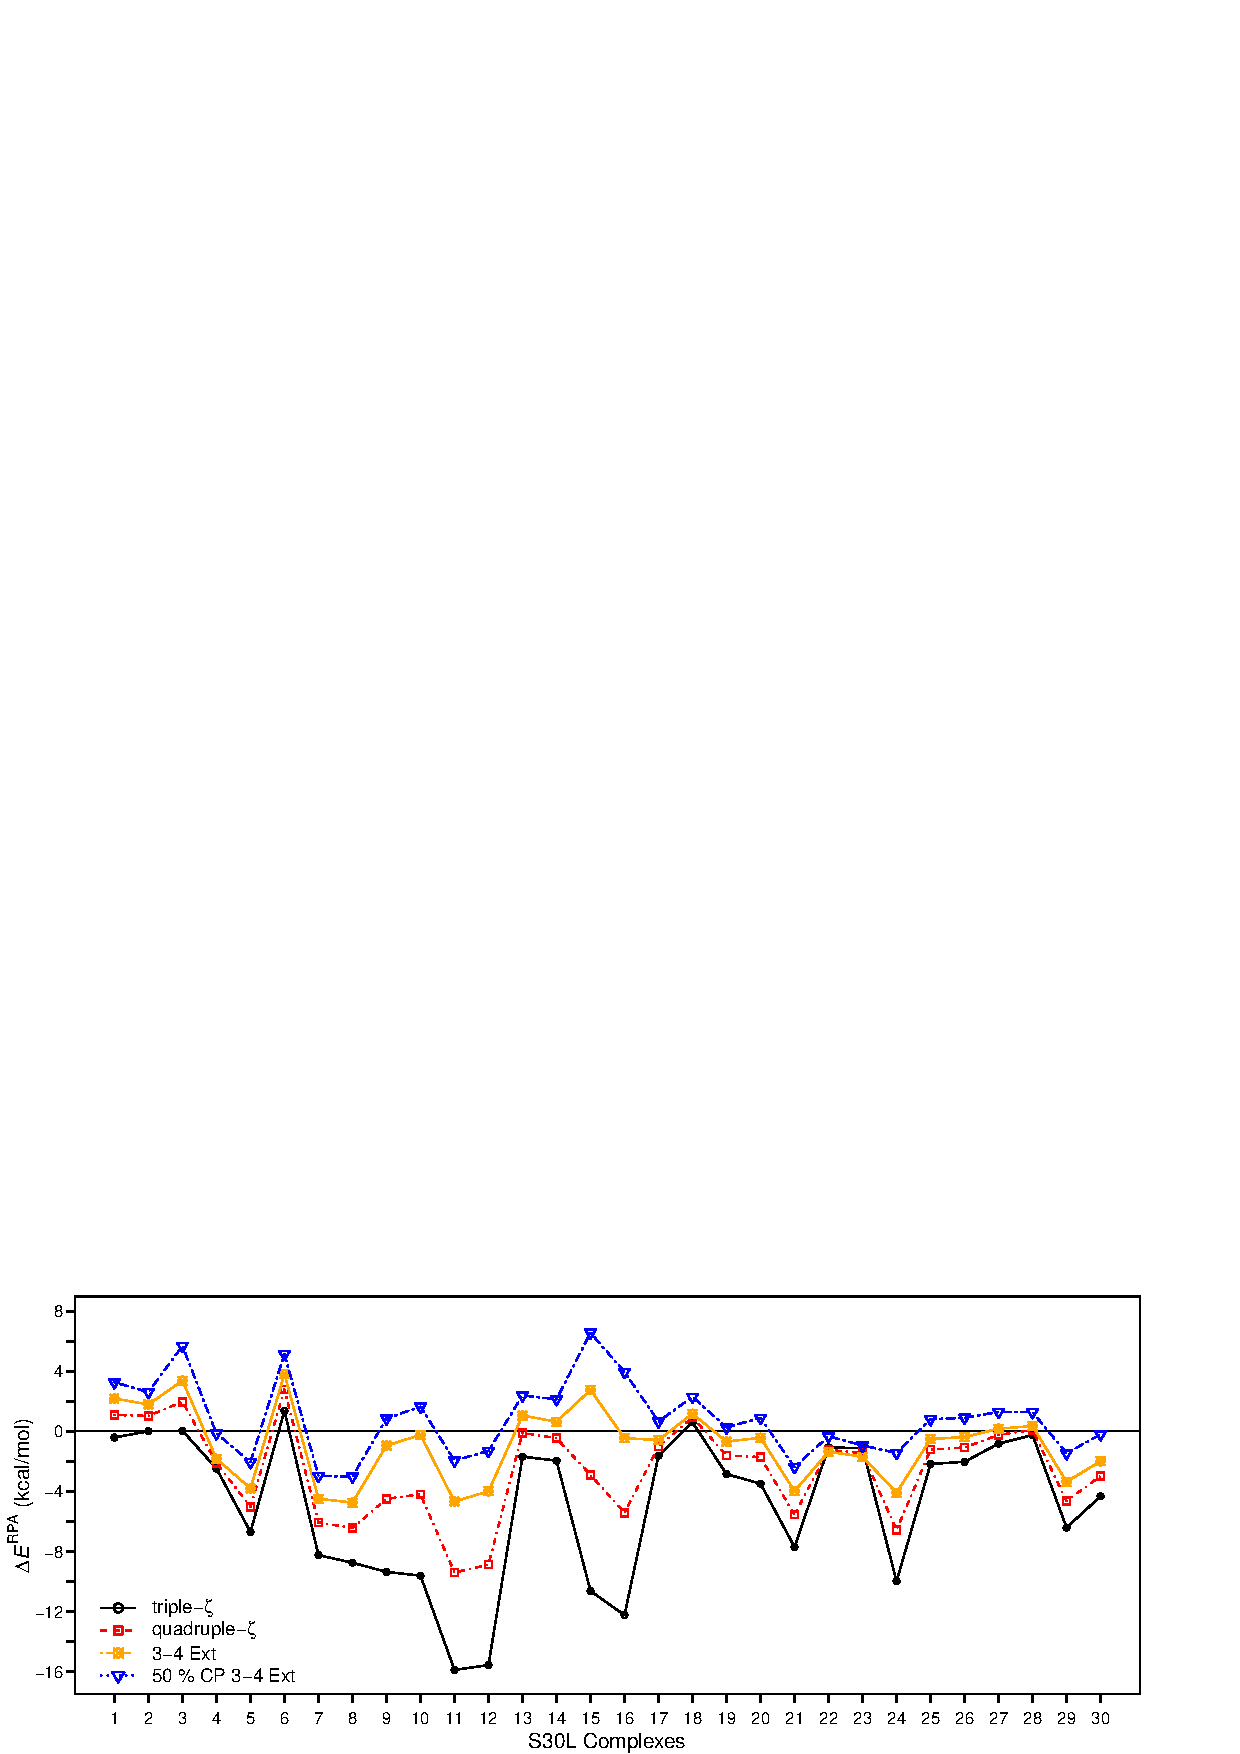
\includegraphics[scale=0.22]{conv_v5}
  \caption{The computed RPA(PBE) interaction energy errors of the
    S30L test set using triple-$\zeta$ basis, quadruple-$\zeta$ basis,
    and triple-quadruple (3-4) $\zeta$ extrapolation procedure with and
    without counterpoise correction.}
  \label{fig:conv}
\end{figure}

Accurate RPA calculations of NI energies require CBS extrapolations
\cite{Eshuis12JChemPhys136p084105}. This is consistent with the
observation that CBS extrapolation systematically corrects RPA
interaction energies for S30L (Fig. \ref{fig:conv}).
It was ascertained in exploratory calculations that increasing the
Dunning's basis sets to cc-pV5Z may lead to further improvement but
at the cost of efficiency, see Fig SI. In comprison to the ROT34,
equilibrium structures are generally less sensitive to basis set
incompleteness error than energies. Increasing the basis sets from
def2-TZVP to def2-QZVP yields a small but systematic decrease in
the error in the RPA rotational constants, see supporting information. %\filipp{Which Table/Figure?}
 
%\begin{figure}[h]
%  \centering
%  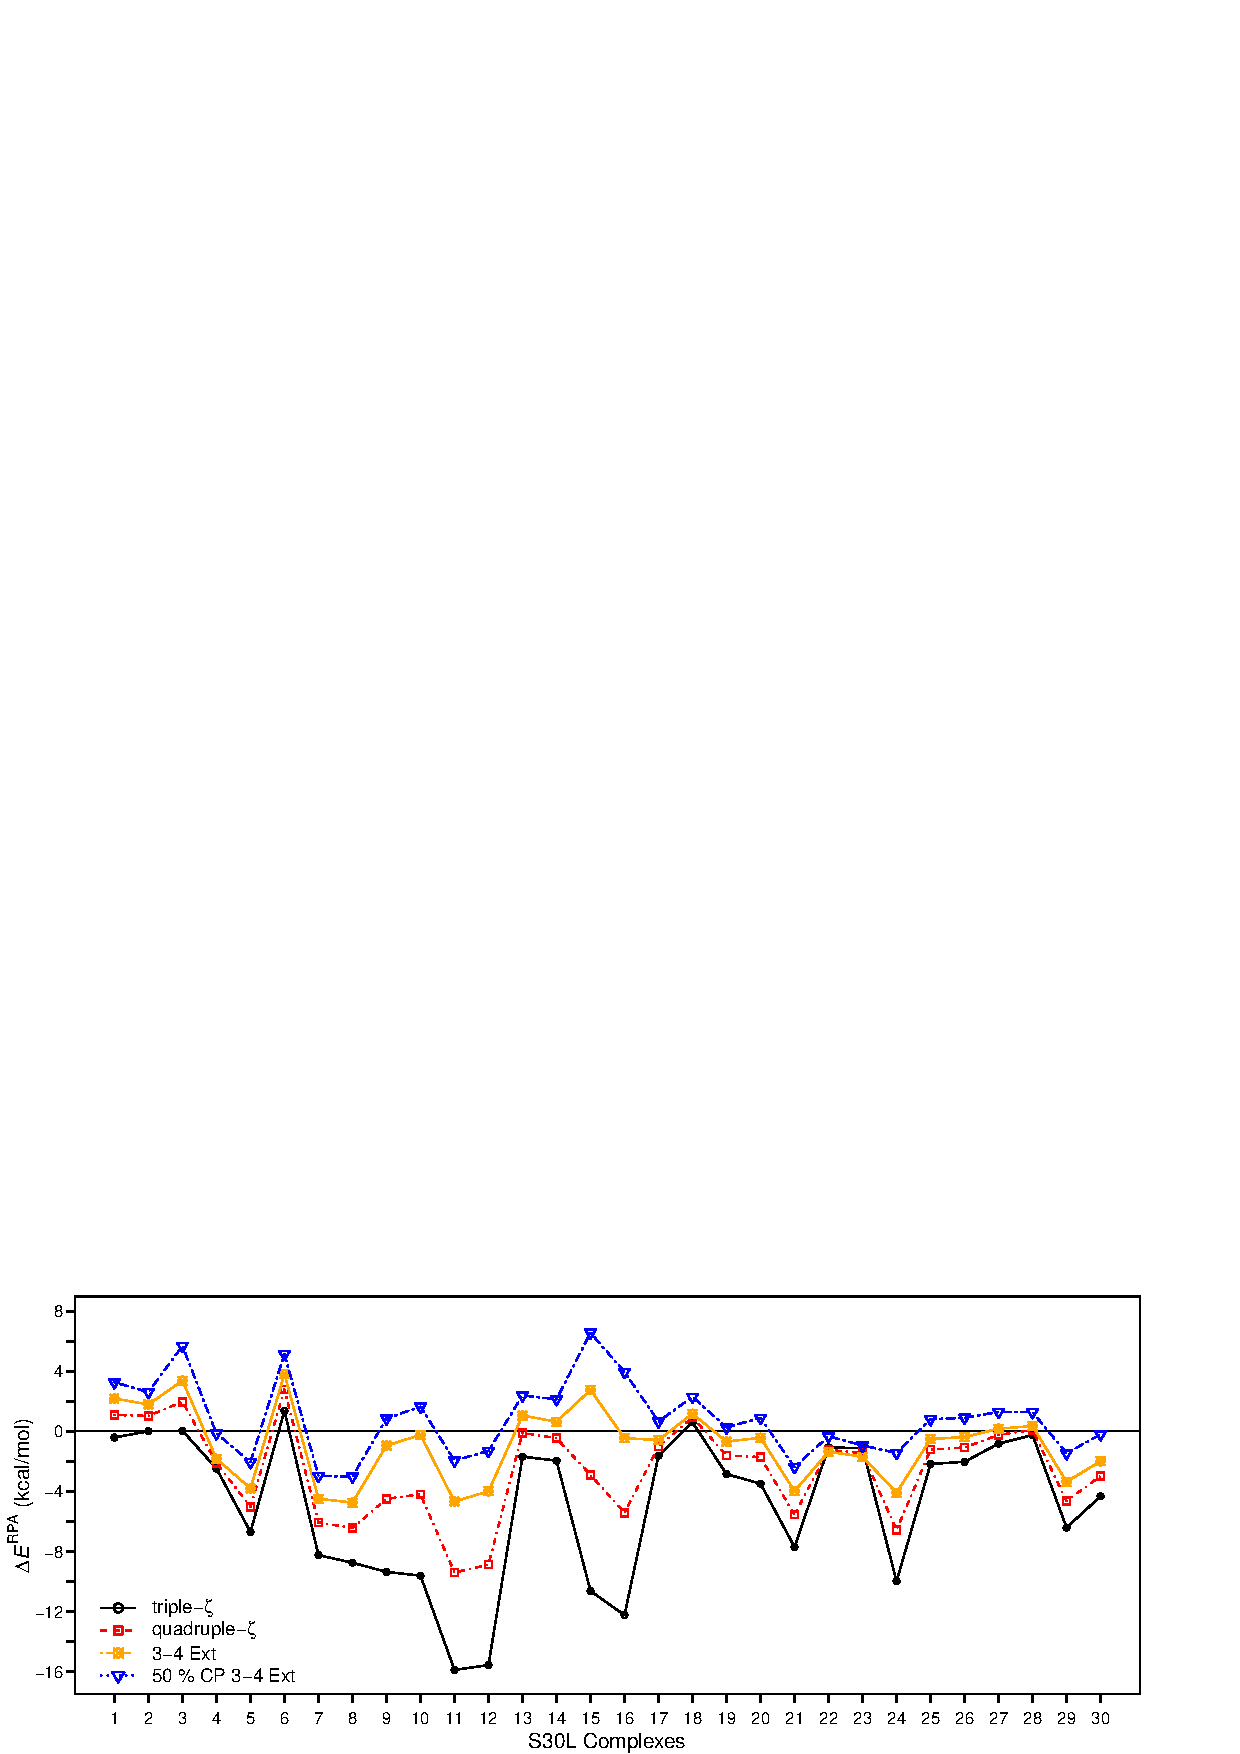
\includegraphics[scale=0.33]{conv_v5}
%  \caption{Basis set convergence of the RPA binding energies for
%    complex 3a of S12L test set with counterpoise correction
%    applied to only the correlation energies. The RPA triple - quadruple zeta
%    extrapolation is denoted as 3-4 RPA.}
%  \label{fig:cp_corrected}
%\end{figure}

\section{Results and Discussion}

\subsection{S30L}

The S30L benchmark revealed the issue of using perturbative
methods such as MP2 to predict NIs of large molecular systems. In Fig.
\ref{fig:theories}, MP2 exhibited consistently large errors and has a
mean absolute error (MAE) of 27.28 kcal/mol. SCS-MP2 and SOS-MP2 may improve
the error with MAE of 15.41 kcal/mol and 25.14 kcal/mol, respectively.
In addition, the range of the errors (rMinMax) were consistently large for all
flavors of MP2 (Table \ref{tbl:s30l}) and SOS-MP2 exhibits unusually
large error for complex 28. In particular, MP2 interaction
energies of the $\pi-\pi$ stacking systems (complexes 5-12) significantly
overbinds. These explicitly shows that while MP2 total energy quality
is size consistent, it does not show MP2 having Casimir-Polder size
consistency that are needed to describe many body effects such
as NIs.

\begin{figure}[h]
  \centering
  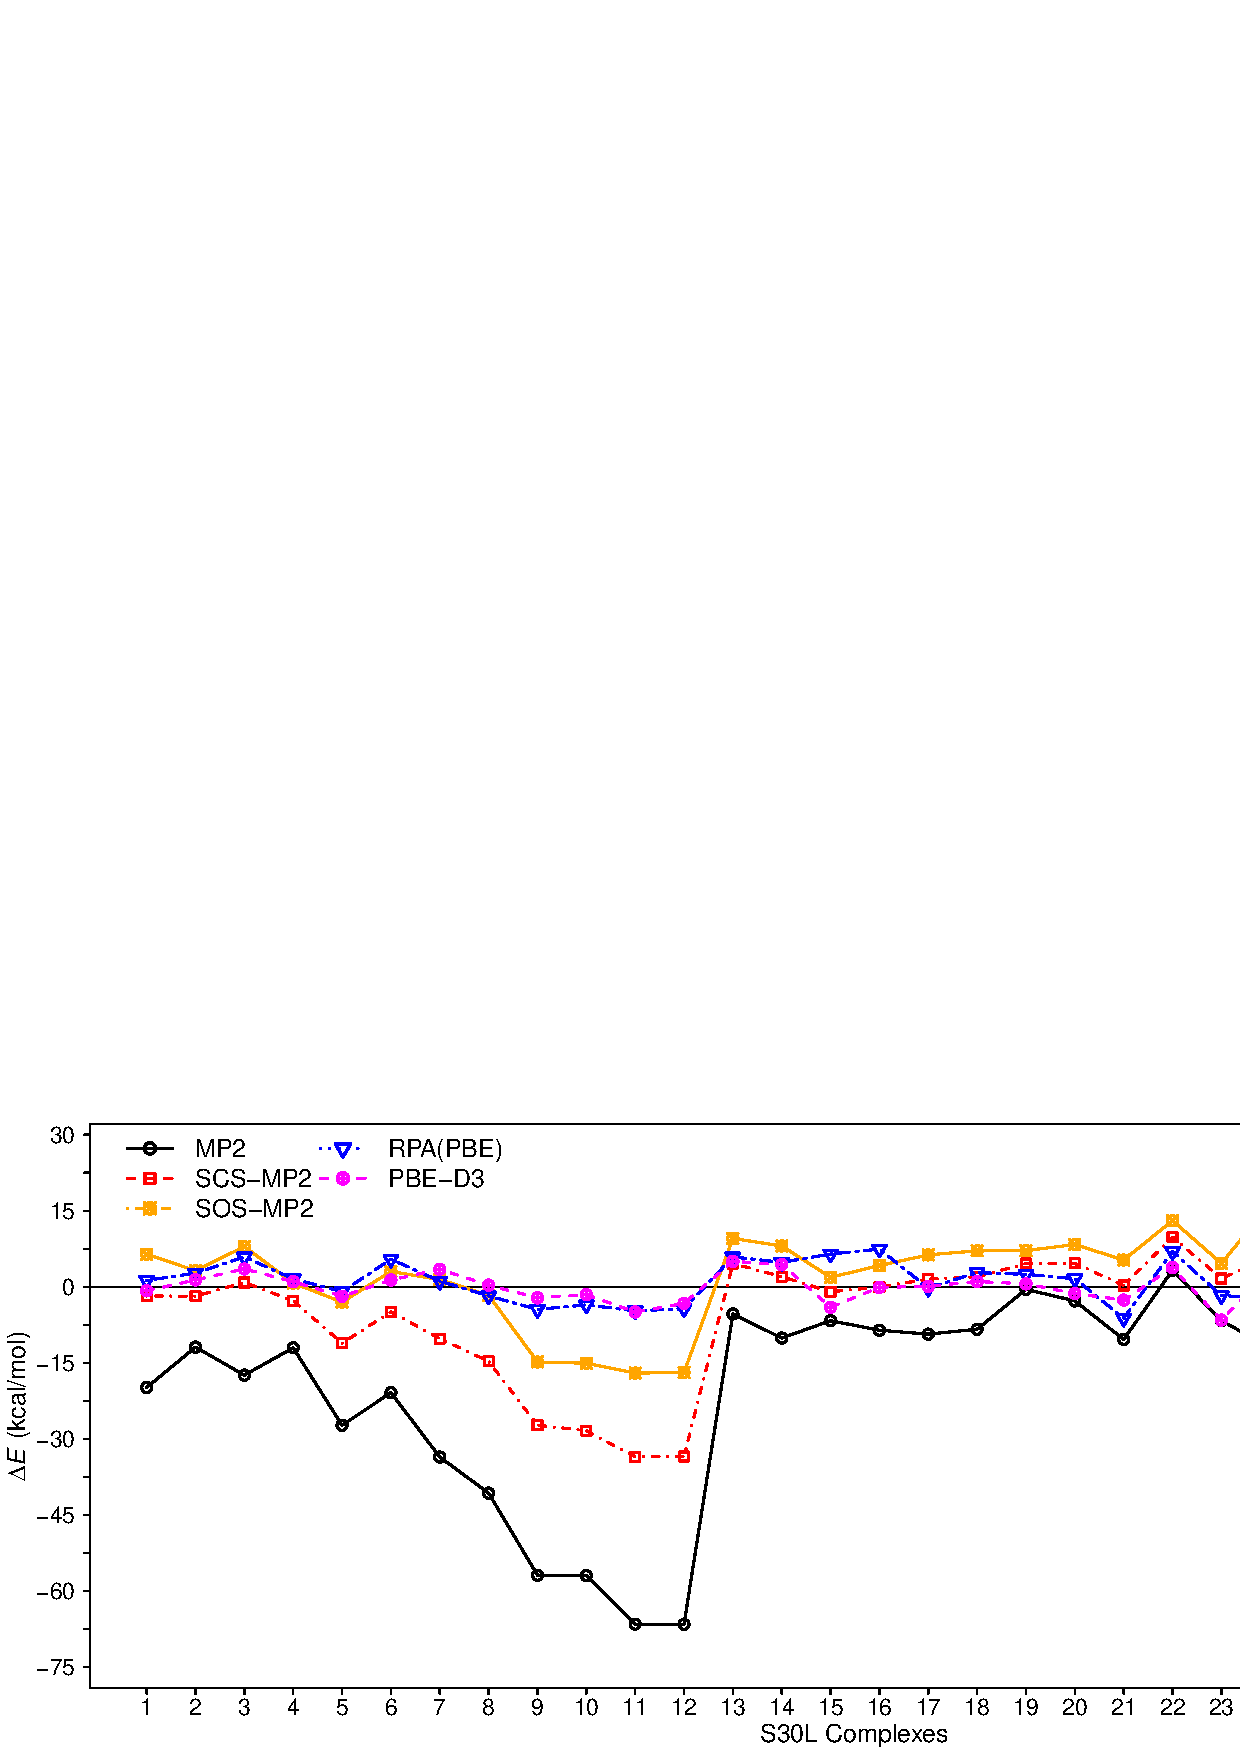
\includegraphics[scale=0.225]{s30l_compare2.png}
  \caption{Deviation of computed S30L interaction energies from
    the reference values \cite{Sure15JChemTheoryComput}.
%    \filipp{Need to state exactly which method uses what basis here}
    PBE-D3 methods with def2-QZVP' were referenced from Sure et
    al\cite{Sure15JChemTheoryComput}. RPA computations treated
    the correlation energy with triple- and quadruple-$\zeta$
    extrapolted Dunning's basis sets and the Hartree Fock exact
    exchange withe Ahlrichs' basis sets.}
%    \filipp{The following should be included in Table 1, not listed in
%      the caption.}}
%    Mean absolute errors for MP2, PBE, PBE-D3, TPSS-D3, RPA(PBE), and
%    RPA(TPSS) are 65.2$\%$, 81.9$\%$, 5.57$\%$, 9.17$\%$, 10.3$\%$, and
%    12.8$\%$, respectively}
  \label{fig:theories}
\end{figure}

In comparison, Random Phase Approximation (RPA) consistently perform
on par with dispersion corrected PBE as seen in Fig \ref{fig:thoeries}.
The accuracy of RPA may slightly depend on the DFT Kohn-Sham reference as shown
by Table \ref{tbl:s30l} where the mean absolute errors of RPA(PBE) and
RPA(TPSS) are 2.51 kcal/mol and 2.77 kcal/mol, respectively.

%Tab. \ref{tbl:s30l}: For compounds 4a and 4b, in the top three with
%most atoms in the benchmark with 148 and 158 atoms, MP2 overbinds 
%by more than 50 kcal/mol, while PBE underbinds by nearly the same
%amount \cite{Grimme12ChemEurJ18p9955,
%  Risthaus13JChemTheoryComput9p1580}. On the other hand, three-body
%empirical dispersion (D3) \guo{(D3 is atom pairwise, so the ``three-body''
%here seems incorrect. Please double check.)} corrected DFAs and RPA yield 
%mean absolute errors of 1-3 kcal/mol. Within the error margins of the
%benchmarks, these methods all perform equally well. 
%
%All methods exhibit much larger deviations for
%cucurbit[7]uril bound with bis(trimethylammoniummethyl)ferrocene 
%(compound 7a) \filipp{I never heard the prefix ``ammonio''. Is this
%  correct?}. \brian{Yes, it is correct} \filipp{seems more common in
%  mineralogoy. Changed.}
%It appears possible that the reference structure, which 
%was obtained at the TPSS-D3/def2-TZVP level, is incorrect. The
%extended S30L benchmark\cite{Sure15JChemTheoryComput} does not contain
%compound 7a; we thus consider it an outlier and do not include it in the
%statistical error analysis.  

\begin{figure}
  \centering
  \includegraphics[scale=0.31]{mp2_rpa_compare.png}
  \caption{These are reported MP2, SCS-MP2, SOS-MP2, and RPA interaction
    energy errors of the L7, S66, and S30L test sets. Energies were
    computed by treating the Hartree exchange with the Ahlrichs basis
    set, and the correlation with the Dunning basis set including 50$\%$
    counterpoise correction and 3-4 extrapolated.}
  \label{fig:mp2_rpa_comp}
\end{figure}

Upon the inclusion of S66 and L7 test sets, the percent error of RPA
remained qualititvely consistent with the size of the system (Fig
\ref{fig:mp2_rpa_comp}). This was not observed with perturbative
methods such as MP2 and SCS-MP2 where the error grows as the system
size grows. The outliers within the MP2 and SCS-MP2 calculations
correspond to $\pi-\pi$ stacking systems which has been known to
be fairly difficult for MP2 to predict NIs. This may pertain to missing
additional higher order terms.

\begin{table}[h]
  \caption{The reported mean absolute errors (MAE) and mean
    errors (ME) in kcal/mol, and relative Min-Max errors (rMinMax)
    in $\%$ for RPA, MP2, SCS-MP2, and SOS-MP2 within the S30L test set.
%    \filipp{The formatting of this table is not consistent with the example above (commented
%      out). Please EXACTLY follow the template.}
  }
  \label{tbl:s30l}
  \setlength{\tabcolsep}{2.7pt}
  \begin{tabular*}{0.48\textwidth}{@{\extracolsep{\fill}}lcccccc}
    \hline
    & RPA(PBE) & RPA(TPSS) & MP2 & SCS-MP2 & SOS-MP2 \\
    \hline
    MAE     & 2.51     & 2.77     & 27.28    & 15.41    & 25.14     \\
    ME      & 0.12     & 1.12     & -27.06   & -9.67    & 7.35      \\
    STDEV   & 3.78     & 3.41     & 29.23    & 26.73    & 54.15     \\
    rMinMax & 37.08    & 23.83    & 387.04   & 327.19   & 313.64    \\
    \hline
  \end{tabular*}
\end{table}

Dispersion is a long range correlation effect that requires higher
order terms to accurately describe NIs as illustrated by Fig \ref{fig:rpa_expand}.
The expansion of the RPA correlation energy of the interaction energy
is shown,

\begin{equation}
  E^{\text{RPA}}_{\text{AB}} - E^{\text{RPA}}_{\text{A}} - E^{\text{RPA}}_{\text{B}}
  = \frac{1}{2}\int^{\infty}_{-\infty} \frac{d\omega}{2\pi}
  \lange \ln(\mathbf{1} - \Pi_{\text{A}}(i\omega)V_{\text{AB}}\Pi_{\text{B}}(i\omega)V_{\text{BA}}) \rangle
  \label{eqn:expand}
\end{equation}

\noindent where $E_{\text{AB}}$, $E_{\text{A}}$, and $E_{\text{B}}$ correspond
to the ground state energies of the complex AB, fragment A, and fragment B,
respectively. By expanding the natural logarithm, it is explicitly shown
that predicting NIs based on perturbation theory will lead to highly
inaccurate results. This can be seen by the highly oscillatory behavior
for higher order terms of weakly interacting systems. In Fig \ref{fig:rpa_expand}
the comparison of helium dimer, benzene dimer, coronene dimer, and
TNF@tweezer2 revealed that the oscillatory behavior grows as the
strength of the NIs increases.

\begin{figure}
  \centering
  \includegraphics[scale=0.13]{rpa_expand3.png}
  \caption{The RPA correlation of the interaction energy is computed at
    nth order of the Taylor series expansion of the EC RPA generates
    intermolecular perturbation series and calculations were performed
    using the PBE Kohn Sham orbital reference with cc-pVTZ basis set.}
  \label{fig:rpa_expand}
\end{figure}
%
%
%\guo{Brian, please also summarize results using def2-TZVP and def2-QZVP and
% state that CBS is necessary.}

\subsection{ROT34}
%
%\guo{Brian, please double check that the sign of the error is defined properly.}
%
%The molecules contained in Rot34 were optimized using RPA with
%PBE\cite{Perdew96PhysRevLett77p3865} and
%TPSS\cite{Tao03PhysRevLett91p146401} reference Kohn-Sham 
%orbitals. \filipp{move this sentence to previous section.}

The ROT34 test set investigates the performance of RPA to account
intramolecular forces. The rotational constants contained in Rot34
range between 454.0 and 4293.9 MHz with an average of 1412.7 MHz, see
SI and Fig. \ref{fig:methods_bar}. Semi-local DFAs such as B3LYP 
yield mean average deviations $>$ 10 Mhz even with dispersion
corrections, although the more recent M06L and SCAN DFAs perform
significantly better\cite{BrandenburgPhysRevB}. The MAE
of MP2 using QZVP basis sets is 5.5 Mhz
\cite{Risthaus13JChemTheoryComput9p1580}, indicating that
intramolecular NPs are challenging for MP2, even for the moderately
sized systems in the Rot34 benchmark. RPA using TPSS reference KS
orbitals almost halves this error to 3.1 Mhz; PBE input orbitals yield
almost identical results. 
%The range of the RPA percentage error is somewhat
%larger, which might reflect its nonvariational character.

 \filipp{Please explain why RPA \% error interval is
  slightly larger, even though ME is small.}

%\begin{table}[htbp]
%  \caption{Rotational constants $B_e$ for RPA(PBE)/TZVP and
%    RPA(PBE)/QZVP-optimized structures displayed as relative
%    deviation in $\%$ from the reference values $B_{ref}$,
%    including mean absolute error (MAE), mean signed error (MSE),
%    and range of Min-Max error (rMinMax) \filipp{Probably move to
%      SI. Need to specify units (MHz)}.}
%{\renewcommand{\arraystretch}{.9}
%\resizebox{!}{.37\paperheight}{%
%    \begin{tabular}{lllcc}
%    \hline\hline
%    Molecule & $B_e$ & $B_{ref}$ &
%    TZVP ($\%$) & QZVP ($\%$)  \\
%    \hline
%    1  Ethynylcyclohexane & A & 4293.9 & -1.31 & -0.07\\
%       & B & 1395.9 & -1.22   & -0.11\\
%       & C & 1129.2 & -1.18   & -0.04\\
%    2  Isoamyl acetate & A & 3322.5 & -1.04 & -0.25\\
%       & B & 719.8  & -0.05   & 0.93\\
%       & C & 698.0  & -0.04   & 1.02\\
%    3  Diisopropyl ketone & A & 3071.1 & -1.28 & -0.22\\
%       & B & 1285.0 & -0.81   & -0.02\\
%       & C & 1248.7 & -1.64   & -0.17\\
%    4  Bicyclo[2.2.2]octadiene & A & 2755.9 & -1.22 & -0.08\\
%       & B & 2675.6 & -1.21   & -0.05\\
%       & C & 2653.3 & -1.18   & -0.12\\
%    5  Triethylamine & A & 2336.9 & -1.52 & -0.20\\
%    6  Vitamin C & A & 1464.2 & -1.54 & -0.66\\
%       & B & 768.2  & -0.80   & 0.27\\
%       & C & 580.6  & -0.83   & 0.12\\
%    7  Serotonine & A & 1165.7 & -1.13 & 0.18\\
%       & B & 661.2  & -0.99   & -0.41\\
%       & C & 454.0  & -1.03   & -0.01\\
%    8  Aspirin & A  & 1166.3  & -2.61 & -0.36\\
%       & B & 767.6  & -0.66   & -0.03\\
%       & C & 767.6  & -1.65   & -0.15\\
%    9  Cassyrane & A & 862.5  & -1.33 & -0.21\\
%       & B & 754.2  & -0.80   & 0.24\\
%       & C & 513.7  & -0.94   & 0.13\\    
%    10 Limonene & A & 3086.2  & -1.28 & -0.12\\
%       & B & 723.7  & -0.95   & 0.13\\
%       & C & 685.0  & -1.26   & -0.13\\
%    11 Lupinine & A & 1432.1  & -1.30 & -0.21\\
%       & B & 820.5  & -1.15   & 0.12\\
%       & C & 679.4  & -1.30   & -0.04\\
%    12 Ac-Pro-NH2 & A & 1523. & -2.43 & -1.08\\
%       & B & 1070.5 & -0.48   & 0.37\\
%       & C & 719.9  & -0.76   & 0.04\\
%    \hline
%    MAE    &    &   &  1.14   & 0.24 \\
%    MSE    &    &   & -1.14   & -0.04    \\
%    rMinMax &    &   & 2.6     & 2.1 \\
%    \hline\hline
%    \end{tabular}}}
%    \label{tab:rot34}
%\end{table}

%\filipp{Compared to B2PLYP-D3,
%  RPA is parameter-free, similar in computational cost, and it may
%  be applied to small-gap compounds such as the Grubbs catalyst
%  or other transition metal compounds (cite Henk's recent paper).}
%[MAKE THIS MORE EXPLICIT].
%[introduce the table and mention which compounds lead to maximum errors]
\begin{figure}[h]
  \centering
  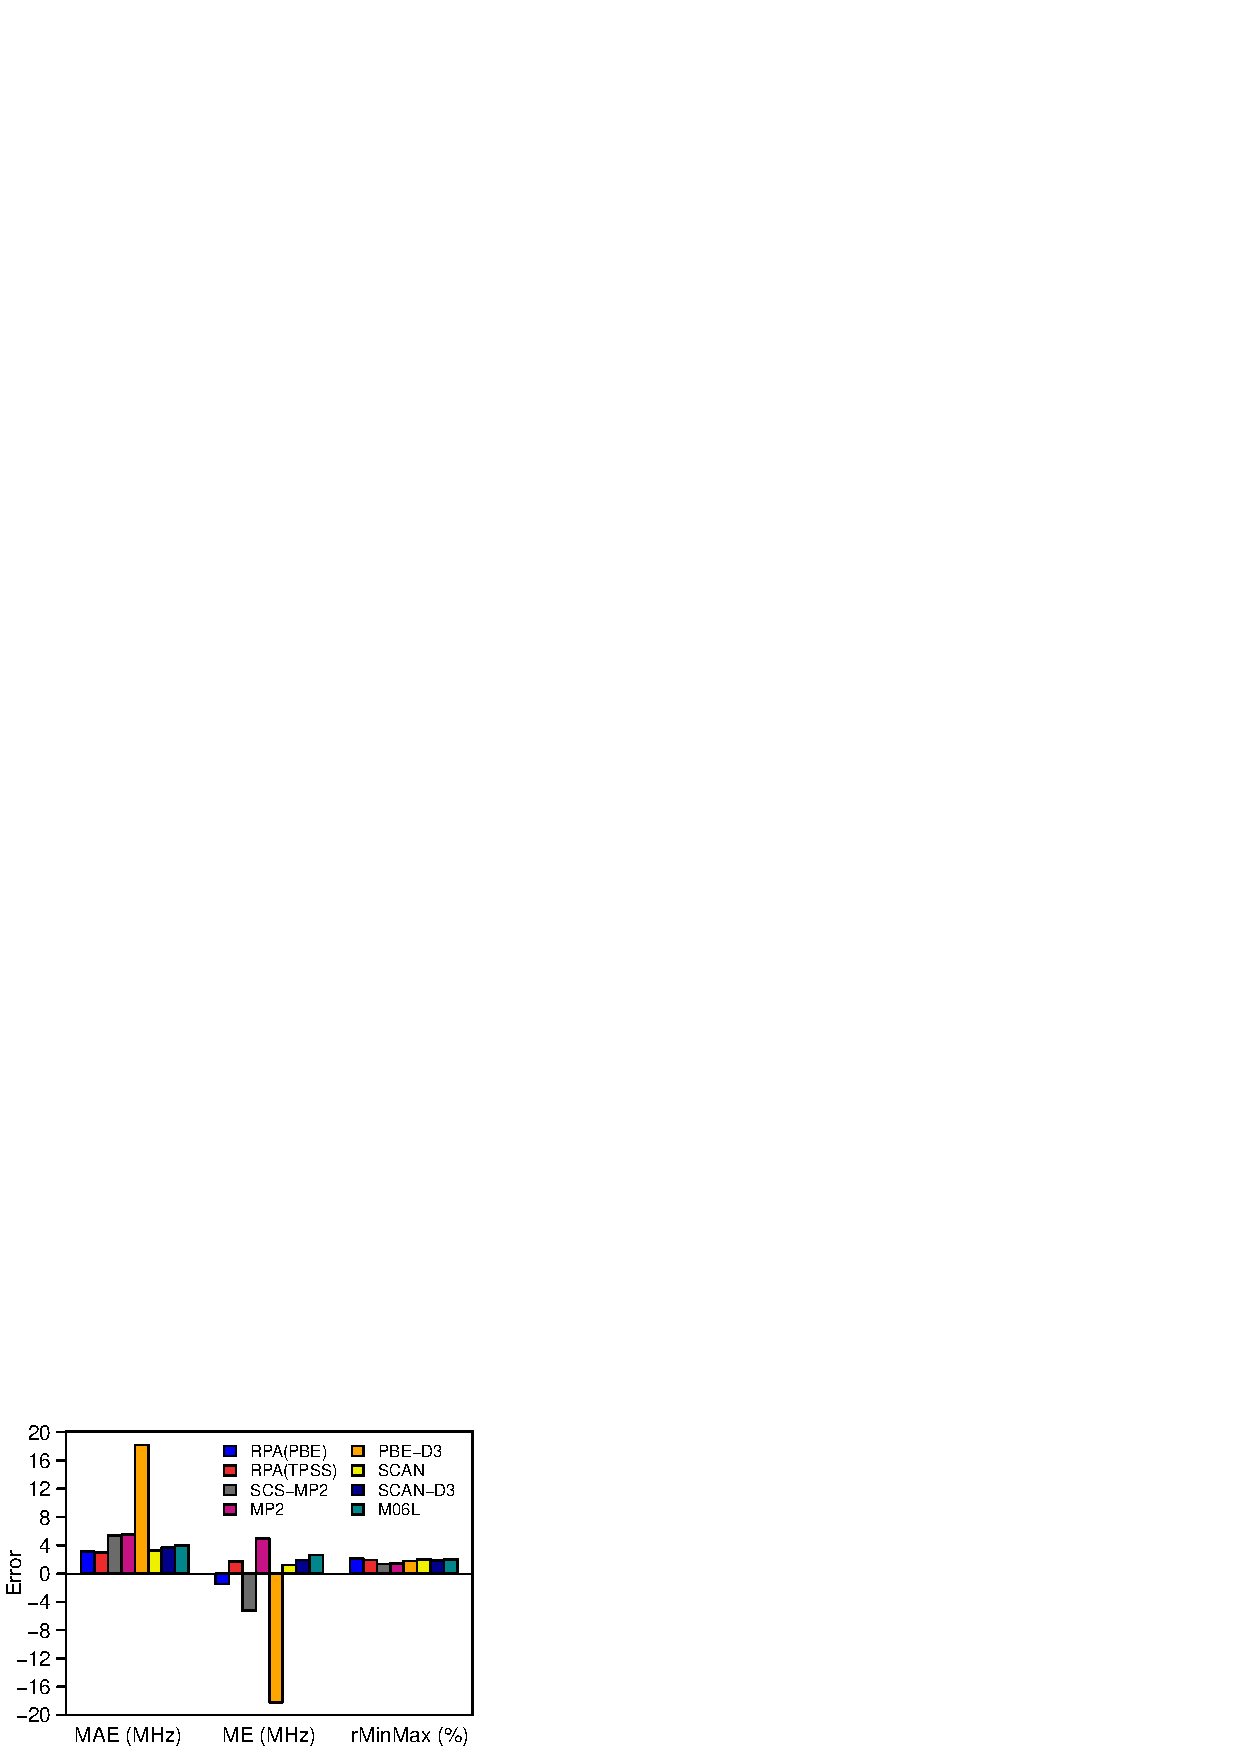
\includegraphics[scale=0.24]{deviate_v4}
  \caption{Statistical analysis of deviations of ROT34 rotational
    constants from experiment
    \cite{Risthaus13JChemTheoryComput9p1580}. Mean absolute errors (MAE)
    and mean errors (ME) are in MHz, and the difference of relative Min-Max errors
%    \filipp{see comments Fig. 3}
    (rMinMax) is in \%. All methods were computed
    with def2-QZVP basis. MP2, DFT, and DFT-D3 referenced from Risthaus et
    al\cite{Risthaus13JChemTheoryComput9p1580}.
%    \filipp{basis set?}
    \filipp{Define all
      abbreviations of methods in Figure, including references if
      necessary. What values are taken from the Literature?} 
%    \filipp{B2PLYP still misspelled in Fig. 4.}
}
  \label{fig:methods_bar}
\end{figure}

\section{Conclusions}

RPA interaction energies for the S30L benchmark exhibit percent error
of approxmately 10$\%$, which is very similar to the errors observed 
for smaller systems \cite{Eshuis11JPhysChemLett2p983}. Relative errors
in rotational constants from the ROT34 set are well below 0.5\%, in line
with previous results for bond lengths in smaller systems
\cite{Burow14JChemTheoryComput10p180,Chen17AnnuRevPhysChem68p421} and
bulk solids.\cite{Harl09PhysRevLett103p056401, Harl10PhysRevB81p115126}
This strongly supports the theoretical expectation that the accuracy of NIs
within RPA should be approximately independent of the system size, and 
contrasts with the performance of MP2 or semilocal DFAs, which severely
deteriorate for large systems. 

Our results further corroborate the argument that missing beyond-pairwise
interactions underly the inconsistent size dependence of NIs within
MP2, and provide a rationale for the good performance of empirical
three- and higher-body dispersion corrections,\cite{Tkatchenko12PhysRevLett108p236402,
  Grimme12ChemEurJ18p9955,DiStasio12ProcNatlAcadSciUSA109p14791} quantum
Drude oscillator models,\cite{Sommerfeld08JPhysChemA112p11021}
as well as approaches such as MP2C.\cite{Pitonak10JChemTheoryComput6p168}
The good performance of RPA compared to MP2 also supports the hypothesis
that electronic structure methods with transferable accuracy need to
include screening.\cite{Bates13JChemPhys139p171103}

RPA long predates the benchmarks studied here, contains no empirically
adjustable parameters (apart from a weak input orbital dependence), and
the two benchmarks were presumably developed without RPA as a specific
target. The level of agreement between RPA and the S30L and Rot34
benchmarks is thus quite remarkable and illustrates the predictive power
of {\it ab initio} electronic structure theory. The more consistent
behavior of RPA as a function of the system size makes RPA preferable to
MP2 for describing NIs even in  moderately large molecular systems with
$\sim$200 atoms, and certainly in condensed matter. While empirical
dispersion corrected DFAs are suitable as cost-efficient first-line
approach, they occasionally fail.\cite{Kim16JPhysChemLett, 
  Hesselmann11PhysChemChemPhys13p732}. RPA calculations are feasible for
systems with hundreds of atoms on workstation
clusters,\cite{Hesselmann12PhysRevA85p012517, Riplinger13JChemPhys,
Kallay15JChemPhys142p204105, Chen17AnnuRevPhysChem68p421, 
Schurkus16JChemPhys144p031101}
%\guo{(How about just ``computer clusters''?
%In 20 or 30 years, people may not know what workstation clusters are.)}
and should be used to calibrate dispersion-corrected DFAs 
for real systems. Further improvements in the accuracy of RPA-type
methods for NIs may be expected from self-consistent generalized Kohn-Sham
RPA calculations,\cite{voora17} which reduce errors in RPA interaction
energies of small molecules by approximately 50\%. 


\section*{Acknowledgment}
This material is based upon work supported by
  the National Science Foundation under CHE-1464828.

\section*{Conflict of interest}

Principal Investigator Filipp Furche has an equity interest in Turbomole
GmbH. The terms of this arrangement have been reviewed and approved by
the University of California, Irvine, in accordance with its conflict of
interest policies. 

%The \balance command can be used to balance the columns on the final page if desired. It should be placed anywhere within the first column of the last page.

\balance

%If notes are included in your references you can change the title from 'References' to 'Notes and references' using the following command:
%\renewcommand\refname{Notes and references}

%%%REFERENCES%%%
\bibliography{references} %You need to replace "rsc" on this line with the name of your .bib file
\bibliographystyle{rsc} %the RSC's .bst file

\end{document}
